\documentclass{report}
\usepackage{a4}
\usepackage{hyperref}
\usepackage{graphicx}
\usepackage{listings}
\usepackage{tabularx}

\usepackage{algorithm}
\usepackage{algpseudocode}
\usepackage{amsmath}
\usepackage{amssymb}
\usepackage{amsthm}
\usepackage{fixltx2e}
\usepackage{graphics}
\usepackage{graphicx}
\usepackage{program}
\usepackage[english]{babel}
\usepackage[T1]{fontenc}
\usepackage[english]{babel}
\usepackage{amsmath,amssymb,amsfonts,textcomp}
\usepackage{color}
\usepackage{calc}
\usepackage{longtable}
\newcommand\textstyleTeletype[1]{\texttt{#1}}

\begin{document}

\title{Exploring Machine Learning:\\
  The ID3 algorithm\\
  		Interim Document}


\author{Mohammed Ibrahim\\
 Computer Science Department\\
  College of Science, Swansea University\\
  Swansea, SA2 8PP, UK
}
\date{}
\maketitle

\tableofcontents

\chapter{File Format}
\label{sec:fileformat}

\section{Introduction}
\label{introd}

This interim document provides the details on the progress made in the project. I have specified details about input and output file format with appropriate examples. My program also calculate the entropy. My documents shows how to calculate the entorpy and I have given an example of calculating entropy.

\section{Input File Format}
\label{sec:file}

A file format is a specific way that information is encoded for storage in a computer file. Each different type of file has a different file format. There are different kinds of file formats for different kinds of information. Some file formats are designed for very particular sorts of data. 
The main objective of having an input file format for our program is that we need the input to be consistent every time the program runs. By having input file format we eliminate the requirement that the program should sort the input attributes in ordered to be processed.
Any input file should follow the following input file format otherwise the program generates the error to the user that the file format is invalid and can't be processed.

\subsection{End-Of-Line}
\label{sec:Eol}


Every file has End-of-line(EOL) symbol and file terminates with the end of line symbol, the end-of-line symbols are invisible.
There are three possibilities including end-of-line symbol in the file.
\begin{enumerate}

\item The programs declares syntax error not having end-of-line symbol.
\item The programs doesn't show any error, it just accept it.
\item The programs displays a warning message stating that there is no end-of-line symbol.

\end{enumerate}

There are 3 line end conventions in common use: CR (MacOS), LF (Unix) and CRLF (Windows). CR 
and LF here refer to characters with ASCII code 13 and 10 respectively. 
Different operating systems use different character sequence to indicate the end-of-line in a text file.
Every single line has end-of-line symbol and it takes 1 byte.


\section{Identifiers}
\label{sec:ide}

According to \cite{Roberts2000CompleteJava2Certification}(Chapter 1, page 6): An identifier is a name used by a programmer to variable, method, package, class, interfaces or label. Keywords and reserved words can't be used as  identifiers. It must begin with a letter, a dollar sign, or an underscore; identifiers are case sensitive. Identifiers are tokens (also called symbols) which name as language entities. Each variable has a name by which it is identified in the program.\\

The input file format rules are:
\begin{enumerate}

\item Comments are ignored in the file by using double slash ($//$) symbol. 
\item Blank line also be ignored in the data file.
\item The attributes and values are separated by using single space.
\item Every file should have end of line.
\item The very first recognizable line of the data file have to be an attributes.
\item The number of attributes is inferred from the number of words in this line.
\item The last word of the attributes is taken as the {\emph target attribute. }
\item In the data file each subsequent line contains the values of attributes for a data point.


\end{enumerate}

\subsection{Restrictions}

Below I have given some restriction, if we doesn't follow the restriction the input file will be invalid. 
\begin{enumerate}

\item We don't allow tab character in the file. If any file contains tab character, we say the file is invalid.
\item Other than double slash ($//$) any other symbol include in the file, we say the file is invalid.
\item Without the end of line symbol we say the file is invalid.


\end{enumerate}

\pagebreak


\subsection{Output File Format}

Below I have specified the output file format for my program.\\

Assume, ``A" is a set of attributes.

A =  ( $a_1, a_2  ,................. a_n$ )

The attribute $a_i$ is the $i^{th}$ attribute in the set ``A".\\

Assume, ``V" is a set of values.

V = ( $v_1, v_2  ,................. v_k$ )

The value $v_j$ is the $j^{th}$ value in the set of ``V".\\

Further, ``T" is the \emph Target Attributes whose values will be boolean 
$T \vee F$


\begin{program} 

	\IF(a_i = v_j) ∧\wedge (a_i+1 = v_j+1) then
	
			T=  T \vee F                                      

\end{program}

Our program will produce an output in the form of if,else clause. The general form of output is given above.
If an attributes value pair satisfies the condition, then the target attribute will have boolean values.\\

The below I have given an example output from the given training set  \ref{fig:trainingplaytennis}.

\begin{lstlisting}

if( outlook == ``sunny") {
	if( humidity == ``high") {
			play = ``no";
	} else if( humidity == "normal") {
			play = "yes";
	}

}
\end{lstlisting}
\pagebreak


\section{Decision Tree}
According to \cite{Mitchell1997MachineLearning}(page 59,Chapter 3): Training set : In machine learning training sets are generally called as tables, where each row in the table represents a single training example. 

To illustrate the operation of ID3, we consider the learning task represented by the example training set given in Figure \ref{fig:trainingplaytennis}. We have four attributes Outlook, Temperature, Humidity and Wind. The target attribute is called PlayTennis, which has values boolean value \texttt{yes} or \texttt{no} for different Saturday mornings, is to be predicted based on other attributes of the morning in question.
\begin{figure}[h]
  \centering
  \begin{tabular}{|c|l|l|l|l|l|l|}
    \hline
    Day & Outlook & Temperature & Humidity & Wind & PlayTennis\\
    \hline
    1 & sunny & hot & high & weak & no
    \\\hline
    2 & sunny & hot & high & strong & no
    \\\hline
    3 & overcast & hot & high & weak & yes
    \\\hline
    4 & rain & mild & high & weak & yes
    \\\hline
    5 & rain & cool & normal & weak & yes
    \\\hline
    6 & rain & cool & normal & strong & no
    \\\hline
    7 & overcast & cool & normal & strong & yes
    \\\hline
    8 & sunny & mild & high & weak & no
    \\\hline
    9 & sunny & cool & normal & weak & yes
    \\\hline
    10 & rain & mild & normal & weak & yes
    \\\hline
    11 & sunny & mild & normal & strong & yes
    \\\hline
    12 & overcast & mild & high & strong & yes
    \\\hline
    13 & overcast & hot & normal & weak & yes
    \\\hline
    14 & rain & mild & high & strong & no
    \\\hline
  \end{tabular}
  \caption{Training set for \texttt{PlayTennis} example}
  \label{fig:trainingplaytennis}
\end{figure}

The below figure shows that the ID3 builds a decision tree from a fixed set of training set examples \ref{fig:decisiontree}. The resulting of the tree is used to classify future samples. The example has several attributes and also called predicted attribute such as :(Outlook, Temperature, Humidity and Wind) and it belongs to a class(target attribute) like ``yes" or ``no". Leaf nodes of the decision tree include the class name whereas a non-leaf node is a decision node. The decision node is an test attribute with each branch (to another decision tree) being a possible value of the attribute. The below tree classifies the Saturday mornings according to whether or not they are suitable for playing tennis.





\begin{figure}[h]
\centering
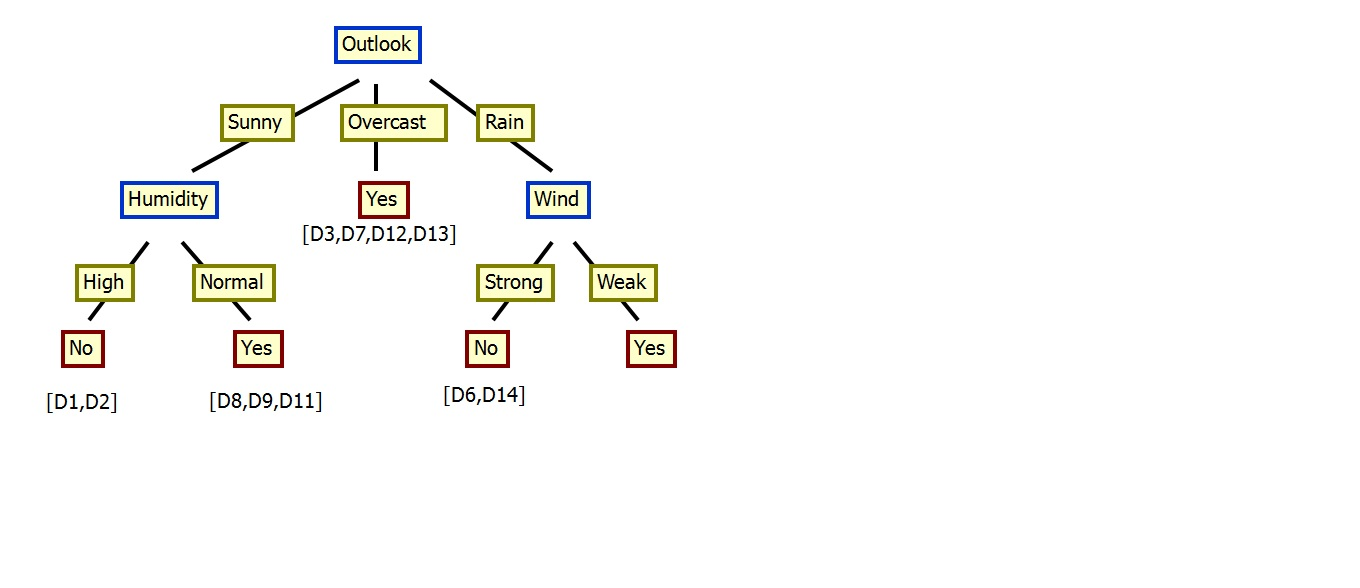
\includegraphics[bb=0 0 1360 588,scale=0.5,keepaspectratio=true]{DecisionTree.jpg}
\caption{Decision Tree}
\label{fig:decisiontree}
\end{figure}


ID3 algorithm uses information gain to decide and to help which attribute goes into a decision node. The central choice in the ID3 algorithm is selecting which attribute to test at each node in the tree. We select the attribute which which is most useful for classifying examples. 
We will define a statistical property, called {\emph information gain } that will measure how well a given attribute separates the training examples according to their target classification.  The ID3 algorithm uses the information gain measure to select among the candidate attributes at each step while growing the tree.
%
%{\centering
%\foreignlanguage{english}{Entropy(S) =
%}\foreignlanguage{english}{${\Sigma}$}\foreignlanguage{english}{
%{}-p(I) log2 p(I)} 
%\par}

{\centering
 $\mathit{Entropy}(S)=\sum -p_i\log _{2}p_i$ 
\par}


Where p(I) is the proportion of S belonging to class I. Σ is over c. Log2 is 
log base2.\\
Note that S is not an attribute but the entire sample set.\\

If S is a collection of 14 examples with 9 YES and 5 NO examples then\\

{\centering
Entropy(S) = {}- (9/14) Log2 (9/14) {}- (5/14) Log2 (5/14) = 0.940
\par}


Notice entropy is 0 if all members of S belong to the same class (the
data is perfectly classified). \\
The range of entropy is 0 (perfectly classified) to 1 (totally random).\\

Gain(S, A) is information gain of example set S on attribute A is
defined as

{\centering

Gain(S, A) = Entropy(S) {}- ${\Sigma}$
(({\textbar}S\textsubscript{v}{\textbar} / {\textbar}S{\textbar}) *
Entropy(S\textsubscript{v}))
\par}

Where:

${\Sigma}$ is each value v of all possible values of attribute A

S\textsubscript{v} = subset of S for which attribute A has value v

{\textbar}S\textsubscript{v}{\textbar} = number of elements in
S\textsubscript{v}

{\textbar}S{\textbar} = number of elements in S

\subsection{Information gain measures}

Suppose S is a set of 14 examples in which one of the attributes is wind
speed. The values of Wind can be \textit{Weak} or \textit{Strong}. \\
The classification of these 14 examples are 9 YES and 5 NO. For attribute
Wind, suppose there are 8 occurrences of Wind = Weak and 6 occurrences
of Wind = Strong. For Wind = Weak, 6 of the examples are YES and 2 are
NO. For Wind = Strong, 3 are YES and 3 are NO.\\ 
\pagebreak

Therefore:

{\centering
\textstyleTeletype{Gain(S,Wind)=Entropy(S){}-(8/14)*Entropy(S}\textsubscript{weak}\textstyleTeletype{){}-(6/14)*Entropy(S}\textsubscript{strong}\textstyleTeletype{)}
\par}

\textstyleTeletype{= 0.940 {}- (8/14)*0.811 {}- (6/14)*1.00}

\textstyleTeletype{= 0.048}

Entropy(S\textsubscript{weak}) = \textstyleTeletype{{}-} (6/8)*log2(6/8)
{}- (2/8)*log2(2/8) = 0.811

Entropy(S\textsubscript{strong}) = \textstyleTeletype{{}-}
(3/6)*log2(3/6) {}- (3/6)*log2(3/6) = 1.00\\

For each attribute, the gain is calculated and the highest gain is used
in the decision node.


\begin{itemize}

\item The idea of decision tree is sorting them down the tree from the root to leaf node, which will provide the classification of instance.
\item Each node in the decision tree states the some attribute of the instance.
\item Each branch descending from that node corresponds to one of the possible values of this attribute.
\item An instance is classified by starting at the root node of the tree,testing the attribute specified by this node, then moving down the tree branch corresponding to the value of the attribute in the given example.
\item This process is repeated for the sub tree rooted at the new node

\end{itemize}

The decision tree is constructed using the techniques of ID3 algorithm. The following steps should follow to construct the decision tree.

According to the book of \cite{Mitchell1997MachineLearning} (page 56, chapter 3) ID3(Examples, target-attribute, attribute)
\begin{itemize}
\item Examples : are the training examples \ref{fig:trainingplaytennis}
\item target-attribute : is the attribute whose value is to be predicted by the tree.
\item Attributes : is a list of other attributes that may be tested by the learned decision tree.\\
Returns a decision tree that correctly classifies the given examples.\\
\end{itemize}


\begin{tabbing}
Create a root node for the tree\\
If \= all examples are positive, Return the single-node tree Root, with label = +.\\
If \= all examples are negative, Return the single-node tree Root, with label = -.\\
If \= Attributes is empty, Return the single-node tree Root, with label = most common value of\\ target attribute in Examples\\
Otherwise Begin \\
\> then \=  A = The Attribute that best classifies examples.\\
\> Decision Tree attribute for Root = A.\\
\> For each possible value, vi, of A,\\
\> \> Add a new tree branch below Root, corresponding to the test A = vi.\\
\> \> Let Examples(vi) be the subset of examples that have the value vi for A\\
\> \> If Examples(vi) is empty\\
\> \> Then below this new branch add a leaf node with label = most\\
\> \> common target value in the examples\\
\> \> Else below this new branch add the subtree ID3 \\
\> \> (Examples(vi), target attribute, Attributes – {A})\\

end\\
return Root\\
\end{tabbing}

\section{Second Example}
Below training set viewed as a set of examples, where each line states the values of certain attributes and a conclusion(Target attribute in our case).

Training set : \cite{RuleInduction}(Page 1):

\begin{figure}[h]
  \centering
  \begin{tabular}{|c|l|l|l|l|l|l|}
    \hline
   Slno & Skin	& Colour & Size & Flesh & Conclusion\\
    \hline
    1 & hairy &	brown &	large &	hard & safe	
    \\\hline
    2 & hairy & green & large & hard & safe
    \\\hline
    3 & smooth & red & large & soft & dangerous
    \\\hline
    4 & hairy & green & large & soft & safe	
    \\\hline
    5 & hairy &	red & small	& hard	& safe
    \\\hline
    6 & smooth & red & small & hard & safe	
    \\\hline
    7 & smooth & brown & small & hard &	safe	
    \\\hline
    8 & hairy &	green &	small &	soft & dangerous	
    \\\hline
    9 & smooth & green & small & hard &	dangerous
    \\\hline
    10 & hairy & red & large & hard & safe
    \\\hline
    11 & smooth & brown & large & soft & safe	
    \\\hline
    12 & smooth	& green & small	& soft	& dangerous
    \\\hline
    13 & hairy	& red & small & soft & safe	
    \\\hline
    14 & smooth	& red &	large &	hard & dangerous
    \\\hline
    15 & smooth & red & small &	hard & safe
    \\\hline
    16 & hairy & green & small & hard & dangerous		
    \\\hline               
                     
  \end{tabular}
  \caption{Training set for \texttt{FoodExample} example}
  \label{fig:foodexample}
\end{figure}

In the other hand, it can be viewed as a set of rules. say an example from the first line:
 

\begin{lstlisting}
if skin = hairy
   and  colour = brown
   and  size = large
   and  flesh = hard
   then conclusion = safe    
    
\end{lstlisting}
Such rules are not constrained to have a fixed number of preconditions. Suppose that there was a rule which had no precondition about the size of the fruit. Then it could be replaced by two rules (there are two possible values for size), that is, one in which size = large and one in which size = small were extra preconditions, or it could be replaced by a rule with the single equivalent extra precondition size = Anything or the precondition (size = large or size = small).
The general form of decision tree for above example:

\begin{lstlisting}

 if attribute1 = value1 then <subtree 1>
   else if attribute1 = value2 then <subtree 2>
   
   else if attribute1 = valueN then <subtree N>

\end{lstlisting}

\chapter{Progress}
\label{cha:pro}

\section{Implementation}
 
The first program ``ComputeDecisionTree" is partially working with the specified file format. My first program only reads the input file (Training set) and produce the decision tree in the form of if, else clause in a separate file. I have collected totally 15 examples input file to test my first program, some files are valid and invalid. If the file is valid according to our specified file format the program computes the decision tree. If any examples file doesn't match according to our specified file format   the output of the program appears as invalid file.
My program also calculate the entropy by using the given formula and in other file it includes the ``Statistics".The statistics contained within the second file will include information such  size of complete table, comparison of the size of the training set and size of the decision tree.

\chapter{project progress Schedule}
\label{cha:pro}


\begin{figure}[h]

\centering
%\includegraphics[bb=0 0 1325 470, scale=0.3, keepaspectratio=false]{../../Ganttchart.png}
\includegraphics[width = 6.5in]{../../Ganttchart.png}
\caption{Gantt Chart}
\end{figure}


\chapter{Re-evaluation of Risks }
\label{cha:risk}

\section{Risks}
\label{sec:risks}

I have details the risks laid out in a table. Severity, chance of occurrence and ability to detect an I have calculated that in scores that 1 and 10.
1 is being almost no chance of occurring or easy to detect. 10 being will defiantly occur and it is almost impossible to detect.
Severity is the impact the risk will have on the project should it come to fruition, chance of occurring is the likely hood the risk will occur and finally ability to detect is based on how fast we can identify and contain the cause of the risk.
The Risk Priority Number (RPN) is calculate by multiplying the severity, chance of occurring and ability to detect together, this number is then we used to rank the risk in order of damage they could potential do to the project allowing us to identify the risk which we must be most aware of, the higher the number the higher the risk.
\pagebreak

\subsection{General Risks}

\begin{table}[h]

\begin{tabularx}{\textwidth}{|X|X|X|X|X|}
\hline 
  Risk & Severity & Change of ocurring & Ability to Detect & Risk Priority Number (RPN)
\\\hline
Short Term illness - The project progress rate could be
slowed for a short period of time.&
3&
2&
10&
40\\\hline
Family Situation - Unplanned events could cause a decrease in productivity for a few days.&
5&
2&
10&
100\\\hline
Heavy Coursework Load - Time spent on the project could be considerably reduced when coursework deadlines clash.&
8&
8&
10&
640\\\hline

  \end{tabularx}
  \caption{General Risk Assesment}
  \label{sec:riskas}
\end{table}

\subsection{Technical Risks}
\label{sec:tech}
\begin{table}[h]
\begin{tabularx}{\textwidth}{|X|X|X|X|X|}
\hline 
Risk & Severity & Change of ocurring & Ability to Detect & Risk Priority Number (RPN) \\ 
\hline 
Feature Creep - Extra features that are not in the specification, could be implemented, wasting time and causing core features to be left unimplemented & 5 & 2 & 2 & 20 \\ 
\hline 
\end{tabularx} 
\caption{Technical Risk Assessment}
\end{table}

\section{Risk Assessment}
\label{sec:rskas}

There are two types of risk involved with this project;
\begin{itemize}
\item General Risk
\item Technical Risk
\end{itemize}
The flaw with this risk assessment is that many read with one risk occurring at one time in there mind. In reality multiple risks will strike at the same time. If any of the top  risks occur at the same time, the project will come to a stop, we do not have the time or man power to minimise the affect of the risks. Unfortunately because the primary risk of Heavy Coursework Load is constant, our ability to pick up extra workload is also severely reduced. In short, we cannot minimise the damaged done to the project when multiple high risks strike at the same time.

\subsection{General Risks}
\label{sec:gr}
Short term illness and family situations are out of our control, not possible to predict when either will occur the only real plan for managing either  is to attempt to pick up the extra workload to keep the project on track, ultimately though the project will suffer delays. Heavy coursework load and time management go hand in hand. We cannot predict the amount of work we will be given or the amount of time it could take to complete. This is why it is the highest risk to the project, it can impair our ability to take action against other risks and seriously hamper project progress. 

\section{Conclusion}
\label{sec:con}

The project has been progressing at a steady rate. The first phase is almost completed; Currently working on displaying second file which will contain statistics. I believe the project has made steady progress but due to medical problem last two week couldn't able to any progress. Now I will make sure my project will complete on time. 




\bibliographystyle{plain}
\bibliography{Bibliography}



\end{document}